\section{Eigenschaften einer IDE}

\begin{frame}
\begin{block}{Integrierte Entwicklungsumgebungen (IDE)}
	\vspace{2pt}
	\uncover<+->{
		Die Arbeit mit gewöhnlichen Texteditoren ist auf Dauer sehr mühsam. Daher empfiehlt es sich eine IDE zu verwenden. 
		Das bringt zum u.a. folgende Vorteile: 
		\begin{itemize}[<+->]
			\item Syntax-Highlighting
			\item Code-Inspection
			\item Autocomplete
			\item Geile Shortcuts
			\item Code direkt ausführen
			\item Hilfe bei der Fehlersuche (\emph{Debugging})
		\end{itemize}	
	}
\end{block}
\end{frame}

\section{Installation}

\begin{frame}
\uncover<+->{
\begin{block}{Installation von PyCharm}
	\vspace{2pt}
	\begin{enumerate}
		\item Gehe auf 
		\texttt{https://www.jetbrains.com/pycharm/download} \\
		\item Lade die kostenlose \textit{Community Edition} herunter
		\item Führe den Installer aus und folge der Installationsanleitung
		\item Öffne PyCharm - falls Du gefragt wirst: Importiere \emph{keine} Settings an dieser Stelle
	\end{enumerate}
\end{block}
}

\uncover<+->{
\begin{block}{Wenn alles passt, sollte es etwa so aussehen:}
	\vspace{2pt}
	\begin{center}
		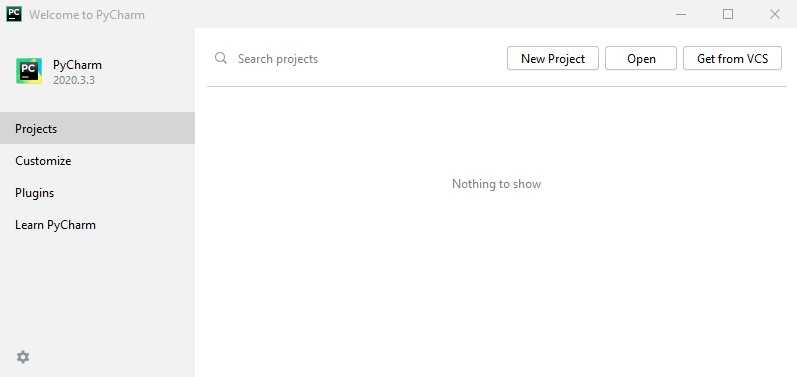
\includegraphics[width=0.65\textwidth]{pycharme.jpg}
	\end{center}
\end{block}
}	
\end{frame}

\section{Konfiguration}

\begin{frame}
\begin{block}{Settings importieren}
\vspace{2pt}
\begin{enumerate}
\item Lade Dir aus der Salem-Cloud die Datei \\ \texttt{Programmieren/Pycharm-Settings/pycharm\_settings.zip} \\ herunter und speichere sie auf Deinem Rechner.
\item Gehe in Pycharm auf \texttt{Customize > Import Settings...}
\item Wähle die zuvor heruntergeladene Datei aus. 
\item Führe einen Restart von Pycharm durch.
\item Falls Du einen Mac hast, stelle unter \texttt{Customize > Keymap} die Keymap \texttt{Salem-Mac} ein. 
\end{enumerate}
\end{block}
\end{frame}
	
\begin{frame}
\begin{block}{Interpreter einrichten}
\begin{enumerate}
\item Öffne Pycharm
\item Wähle \texttt{Project > New Project}
\item Dort kannst Du folgendes einstellen:
\begin{enumerate}
	\item Wähle unter \texttt{Location} einen Pfad, den Du auf Deinem Rechner wiederfindest
	\item Unter \texttt{Base Interpreter} wähle ein Python $\geq 3.6$ (Vorsicht: Der Punkt wird nicht immer mitgeschrieben)
	\item Setze einen Haken unter \texttt{Make available to all projects} 
	\item Setze den Haken unter \texttt{Create a main.py welcome script}
\end{enumerate}
\end{enumerate}	
\end{block}

\pause 

\begin{block}{So könnte es in etwa aussehen}
	
	\begin{center}
		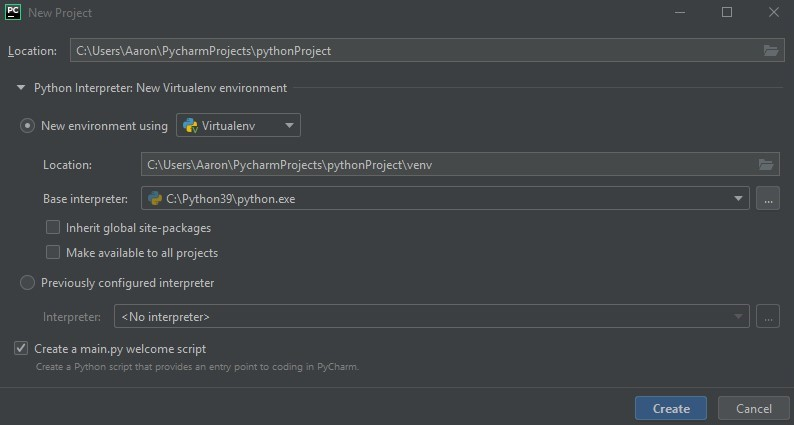
\includegraphics[width=0.5\textwidth]{python_interpreter.jpg}
	\end{center}
	
\end{block}

\end{frame}


\begin{frame}

\begin{block}{Nachdem Du auf \texttt{create} geklickst hast, sollte es etwa wie folgt aussehen}
\vspace{2pt}
	\begin{center}
		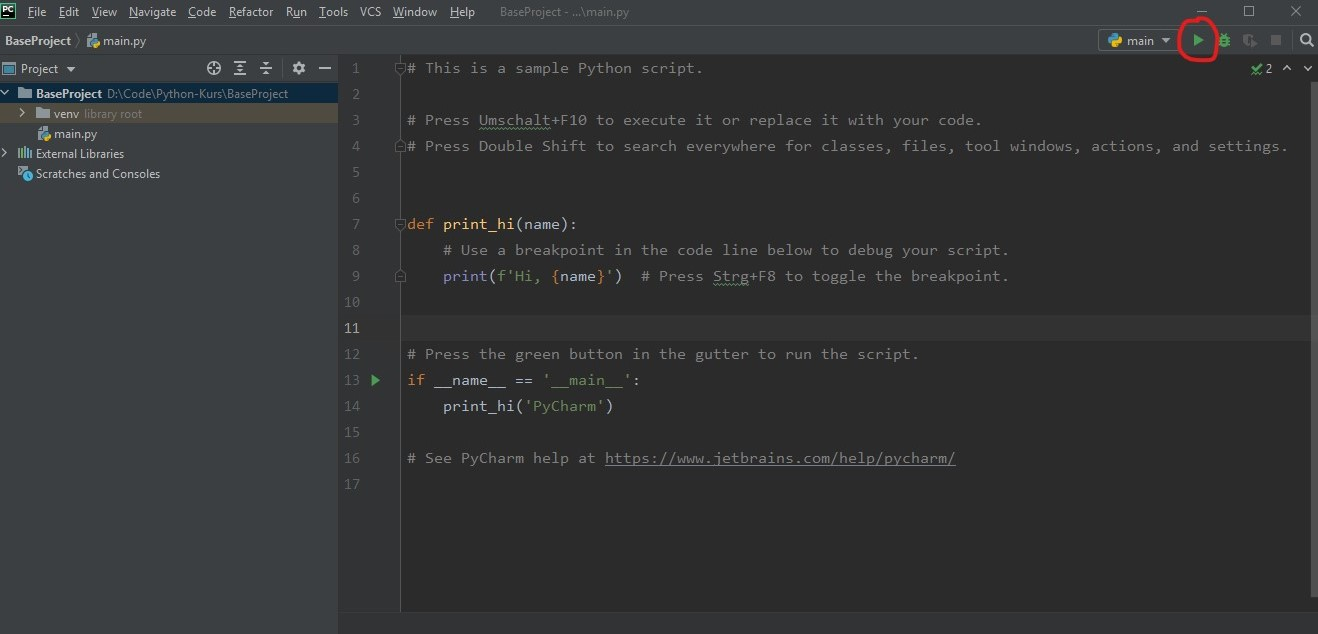
\includegraphics[width=0.85\textwidth]{pycharm_skript.jpg}
	\end{center}	



\end{block}

\end{frame}


\begin{frame}

\begin{block}{Den Code ausführen}
\vspace{2pt}
Klickst Du nun auf den grünen Pfeil oben rechts (siehe roter Kreis), sollte sich eine kleine Konsole öffnen und das Programm ablaufen. 
Alternativ kannst Du auch die Tastenkombination \texttt{Cmd + Enter} (Mac) bzw. \texttt{Strg + Enter} (Windows) verwenden.  

\pause

\begin{center}
	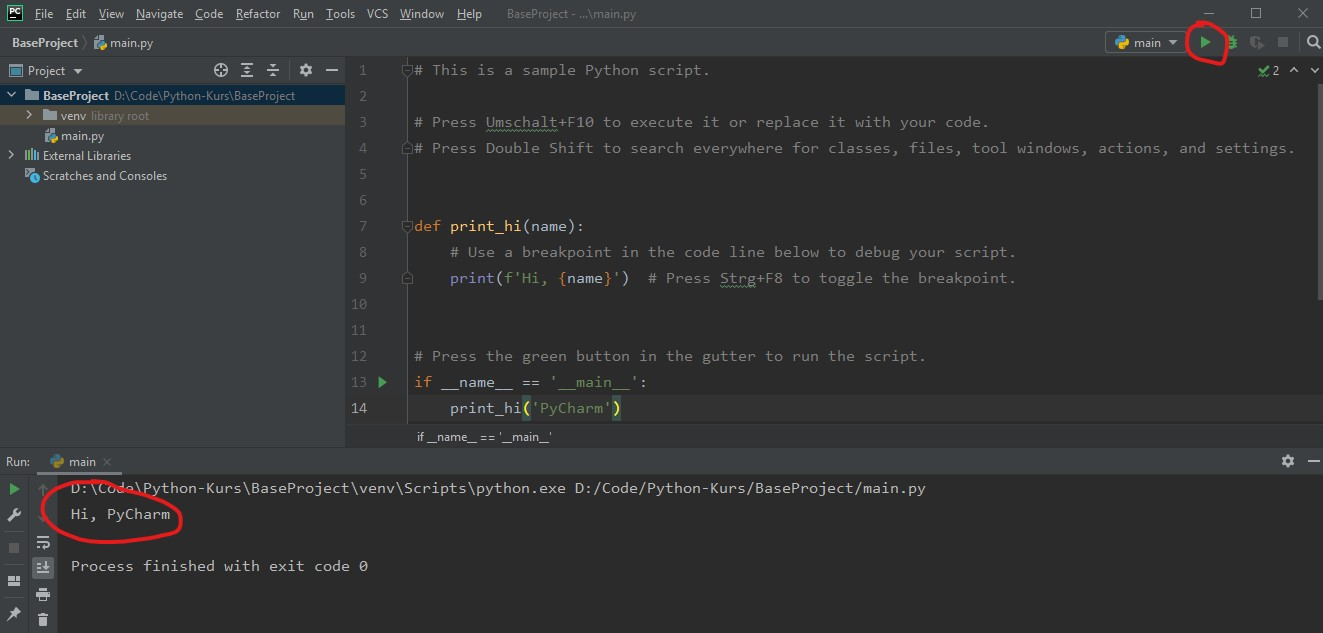
\includegraphics[width=0.85\textwidth]{pycharm_run.jpg}
\end{center}	

\end{block}

\end{frame}

